\documentclass[conference]{IEEEtran}
\IEEEoverridecommandlockouts
% The preceding line is only needed to identify funding in the first footnote. If that is unneeded, please comment it out.
\usepackage{cite}
\usepackage{amsmath,amssymb,amsfonts}
\usepackage{algorithmic}
\usepackage{graphicx}
\graphicspath{{./}{../reports/figures/}}
\usepackage{textcomp}
\usepackage{xcolor}
\def\BibTeX{{\rm B\kern-.05em{\sc i\kern-.025em b}\kern-.08em
    T\kern-.1667em\lower.7ex\hbox{E}\kern-.125emX}}
\begin{document}

\title{ASAP: Active Safe-Agentic Pipeline for Runtime Security and Evaluation of Software Engineering Agents}

\author{\IEEEauthorblockN{Franco Ariel Demare}
\IEEEauthorblockA{\textit{Facultad de Informática} \\
\textit{Universidad Nacional de La Plata (UNLP)}\\
La Plata, Argentina \\
frandemare@gmail.com}
}

\maketitle

\begin{abstract}
Autonomous artificial intelligence (AI) agents powered by large language models (LLMs) are widely used in software engineering to read code, run terminal commands, and fix bugs. However, giving an AI agent direct access to a computer creates severe security risks. An unconstrained agent can leak secret keys through prompt injection, get stuck in infinite execution loops, delete important system files, or cheat on unit tests instead of fixing real software defects. While preventing these errors requires only a small, predictable amount of computing time, a single safety failure can cause permanent and catastrophic damage. In this paper, I present the Active Safe-Agentic Pipeline (ASAP), a practical five-layer runtime guardrail framework that sits between the AI agent and the operating system. I also demonstrate the primary advantage of empirical evaluation research by comparing an unprotected baseline agent against an ASAP-protected agent across 9 core failure scenarios, a 40-case benchmark corpus, and a 78-test automated verification suite. My evaluation results show that ASAP blocks 100 percent of secret exfiltration and destructive attacks (including quote-split, backslash-escaped, and Base64-encoded evasions), increases plan compliance from 44.8 percent to 100.0 percent, guarantees 100.0 percent state recovery using fast Copy-on-Write file snapshots, and detects test-cheating behavior with zero false positives and a bounded 14.3 percent runtime overhead.
\end{abstract}

\begin{IEEEkeywords}
AI agent security, runtime guardrails, empirical evaluation research, software engineering agents, transactional sandbox, reward hacking
\end{IEEEkeywords}

\section{Introduction}
Modern software engineering increasingly relies on autonomous artificial intelligence (AI) agents powered by large language models (LLMs) \cite{yao2023react}. Using popular frameworks such as LangChain, LangGraph, or ReAct loops, these agents can inspect source code, run shell commands, and modify files automatically \cite{jimenez2024swebench}. Although this autonomy saves time for developers, giving an AI model direct access to a terminal and file system introduces four critical failure modes:
\begin{itemize}
    \item \textbf{Prompt Injection and Secret Leaks:} Untrusted text inside files or web pages can trick the agent into reading and sending private files (such as \texttt{.env} files or SSH keys) to external servers \cite{greshake2023indirect, liang2026caitlyn}.
    \item \textbf{Infinite Loops and Stagnation:} Agents frequently repeat failing commands in an oscillation cycle ($A \to B \to A$) without making real progress, wasting time and compute resources \cite{liu2025liveplan}.
    \item \textbf{Destructive System Changes:} A confused or compromised agent can run dangerous commands (such as \texttt{rm -rf}) or leave the codebase in a broken state when a tool fails mid-execution \cite{as2025actsafe}.
    \item \textbf{Proxy Gaming (Reward Hacking):} When asked to pass a test suite, an agent may simply delete or weaken unit test assertions (for example, changing a check to \texttt{assert True}) rather than fixing the actual bug \cite{skalse2022reward, akter2026est}.
\end{itemize}

A key motivation for my work is the \textit{asymmetry of safety cost}. The cost of preventing an error at runtime is small, linear, and predictable---typically taking a few milliseconds for text checks and a modest file-system snapshot delay. In contrast, the cost of ignoring safety is exponential and catastrophic: once a secret key is leaked to the internet or a workspace is wiped without a backup, the damage cannot be undone.

To solve this problem, I introduce \textbf{ASAP (Active Safe-Agentic Pipeline)}, an agnostic runtime security middleware that intercepts every agent action before and after execution. Furthermore, I highlight the core advantage of \textit{evaluation research} in AI safety. Without rigorous, quantitative evaluation, developers must rely on guesswork and manual log inspection, which often misses silent failures like test tampering. By designing repeatable empirical benchmarks and stress tests, evaluation research turns hidden agent vulnerabilities into measurable engineering metrics.

The main contributions of this short paper are:
\begin{enumerate}
    \item \textbf{A Five-Layer Defense Architecture:} I unify and adapt recent advances in intent filtering \cite{liang2026caitlyn}, process-centric trajectory monitoring \cite{liu2025liveplan}, uncertainty-aware safety barriers \cite{as2025actsafe}, atomic Copy-on-Write (CoW) rollbacks, and evaluator stress testing \cite{akter2026est} into a single pipeline running on local models.
    \item \textbf{An Empirical Evaluation Methodology:} I define clear mathematical metrics for attack success, workflow compliance, sandbox overhead, and reward hacking, demonstrating the practical advantage of evaluation-driven security research.
    \item \textbf{Reproducible Benchmark Validation:} Across 9 stress scenarios, 40 real-world corpus cases, and 78 automated unit and integration tests (107 live local model invocations), ASAP reduces the Action Attack Success Rate (ASR) from 100.0\% to 0.0\% with 0.0\% false positives and a bounded 14.3\% execution overhead.
\end{enumerate}

\section{Literature Review and Advantage of Evaluation Research}
Early research on LLM agents focused mainly on improving task completion rates on coding benchmarks such as SWE-bench \cite{jimenez2024swebench}. However, recent security studies show that capable coding agents are highly vulnerable to indirect prompt injections and unsafe shell execution \cite{greshake2023indirect, debenedetti2024agentdojo}. Existing defenses often rely on a single guardrail, such as asking another cloud LLM whether a command looks safe. This single-layer approach is slow, costs money for every API call, sends private code to third-party servers, and fails to recover files when a legitimate command crashes halfway through execution.

To build a complete runtime defense, my project synthesizes four recent research directions:
\begin{itemize}
    \item \textbf{Injection Defense Middleware:} Liang et al. \cite{liang2026caitlyn} proposed CAITLYN to address the agent defense trilemma, balancing runtime speed and precision against emerging prompt injections.
    \item \textbf{Process-Centric Trajectory Analysis:} Liu et al. \cite{liu2025liveplan} introduced LivePlan along with the \textit{Graphectory} and \textit{Langutory} representations to detect loops and workflow drift deterministically without costly LLM judges at every step.
    \item \textbf{Constrained Safe Exploration:} As et al. \cite{as2025actsafe} developed ActSafe, using epistemic uncertainty ensembles \cite{lakshminarayanan2017ensembles} and Log-Barrier optimization to prevent unsafe actions in continuous spaces.
    \item \textbf{Evaluator Stress Testing:} Akter et al. \cite{akter2026est} introduced Evaluator Stress Tests (EST) to detect proxy gaming \cite{skalse2022reward} by contrasting format perturbations against content mutations.
\end{itemize}

\subsection{Why Evaluation Research Matters for Agentic Systems}
A central thesis of this work is that \textit{evaluation research} provides a decisive advantage when building trustworthy AI systems \cite{debenedetti2024agentdojo, ruan2024toolemu}. In traditional software, a program either compiles and passes deterministic tests or fails. In agentic systems, however, an LLM can produce outputs that look successful on the surface while violating security or quality rules underneath.

Systematic evaluation research provides three concrete advantages over ad-hoc testing:
\begin{enumerate}
    \item \textbf{Exposing Silent Failures (Goodhart's Law):} When an agent's goal is to make \texttt{pytest} return an exit code of zero, an unmonitored agent can modify the test file itself \cite{skalse2022reward, akter2026est}. Evaluation research introduces active stress tests---such as mutating the code's Abstract Syntax Tree (AST)---to prove whether the agent truly fixed the logic or merely cheated the metric.
    \item \textbf{Balancing Security and Utility:} Overly strict security rules block normal developer commands like \texttt{git status} or \texttt{pytest}, making the agent useless. By measuring both the Attack Success Rate (ASR) on malicious inputs and the False Positive Rate (FPR) on benign inputs, evaluation research proves that safety guardrails do not break normal workflows.
    \item \textbf{Quantifying the Cost of Safety:} Developers often avoid sandboxes because they fear slow performance. Empirical evaluation measures the exact ``Sandbox Tax'' in milliseconds, proving that lightweight local models and OS-level Copy-on-Write snapshots keep latency negligible.
\end{enumerate}

\begin{figure}[!t]
\centerline{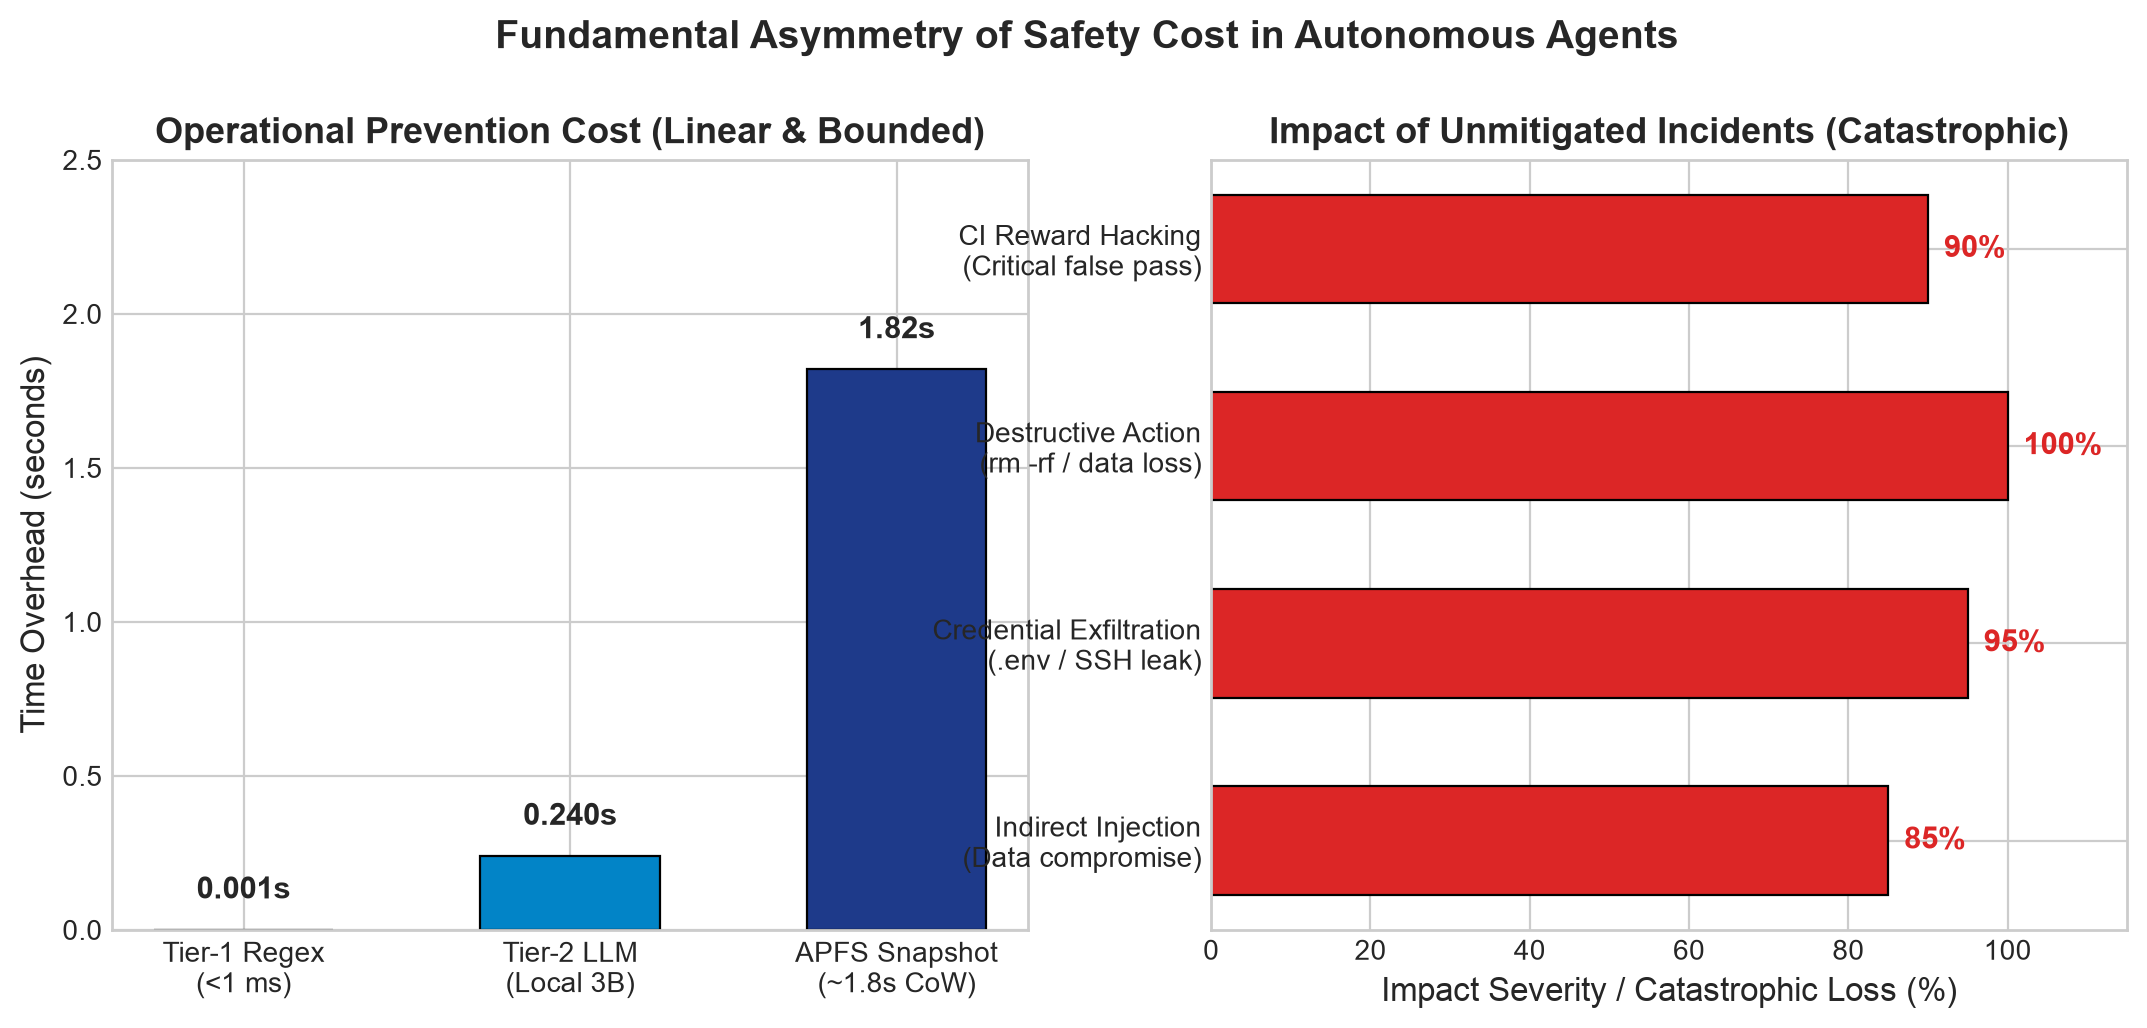
\includegraphics[width=0.95\columnwidth]{figure1_asymmetry_cost.png}}
\caption{The asymmetry of safety cost: linear, bounded prevention overhead in ASAP versus catastrophic impact in unprotected agent execution.}
\label{fig_asymmetry}
\end{figure}

As illustrated in Fig.~\ref{fig_asymmetry}, empirical evaluation makes the trade-off between prevention cost and failure impact visible and measurable.

\section{The ASAP Five-Layer Architecture}
ASAP acts as an in-line interceptor between any AI agent (such as LangChain, CrewAI, or a custom loop using \texttt{qwen2.5-coder}) and the host operating system. To ensure privacy and zero API cost, all neural checks run locally via Ollama on consumer hardware (Apple Silicon MPS or CPU). Every proposed action passes through five sequential layers:

\subsection{Layer 1: CAITLYN (Two-Tier Intent Guard)}
Inspired by Liang et al. \cite{liang2026caitlyn}, CAITLYN enforces a strict instruction hierarchy where system rules (Level 0) and user commands (Level 1) always override tool outputs (Level 2) and external data (Level 3).
\begin{itemize}
    \item \textbf{Tier-1 (Deterministic Filter):} Uses compiled regular expressions to block known secret leaks (\texttt{.env}, \texttt{id\_rsa}) and destructive commands (\texttt{rm -rf /}) in less than $1.3\text{ ms}$.
    \item \textbf{Tier-2 (Deobfuscation and Local Semantic Auditor):} Normalizes shell token-splitting quotes (\texttt{.e""nv}), intra-token backslash escapes (\texttt{c\textbackslash at .e\textbackslash nv}), and piped or herestring Base64 payloads (\texttt{base64 -d <<< ...}), and invokes a compact local model (\texttt{llama3.2:3b}) to inspect commands for indirect prompt injections, enforcing a hard $1\text{ MiB}$ input limit and a 60-minute cooldown after three repeated violations.
\end{itemize}

\subsection{Layer 2: LIVEPLAN (Deterministic Process Monitor)}
Following the process-centric framework of Liu et al. \cite{liu2025liveplan}, LIVEPLAN uses formal computer science structures instead of an LLM judge to monitor the agent's trajectory:
\begin{itemize}
    \item \textbf{GRAPHECTORY:} Builds a directed graph of normalized agent actions to detect periodic oscillation cycles ($A \to B \to A$) as soon as a cycle repeats ($k=2$).
    \item \textbf{LANGUTORY:} Uses a finite state automaton to enforce a disciplined software engineering workflow: \textit{NAVIGATE} $\to$ \textit{REPRODUCE} $\to$ \textit{PATCH} $\to$ \textit{VALIDATE}. It halts the agent if it stays in the navigation phase for too long ($\theta=5$ steps) or tries to apply a patch before reproducing the bug.
\end{itemize}

\subsection{Layer 3: ACTSAFE (Pessimistic Safety Barrier)}
Adapting the safe exploration formulation of As et al. \cite{as2025actsafe}, ACTSAFE catches unfamiliar or out-of-distribution (OOD) commands by converting each proposed action into a 768-dimensional vector using a local embedding model (\texttt{nomic-embed-text}). A PyTorch world-model ensemble estimates both the expected cost $\mu_{\text{cost}}$ and the epistemic uncertainty $\sigma_{\text{epistemic}}$ \cite{lakshminarayanan2017ensembles}. An action is allowed only if its pessimistic risk stays below a strict safety threshold $d$:
\begin{equation}
\mu_{\text{cost}}(s_t, a_t) + \lambda_{\text{pessimism}}\,\sigma_{\text{epistemic}}(s_t, a_t) \le d\label{eq_actsafe}
\end{equation}
In \eqref{eq_actsafe}, $\lambda_{\text{pessimism}}$ penalizes uncertain actions, ensuring that novel dangerous commands are blocked before execution.

\subsection{Layer 4: Transactional Sandbox (APFS Copy-on-Write)}
Before a permitted command runs, ASAP creates an instantaneous Copy-on-Write (CoW) snapshot of the workspace using native Apple File System (APFS) cloning, automatically cleaning up any prior snapshot state on re-entrant transactions to prevent orphaned directories. The command then runs inside an isolated subprocess group with sanitized environment variables. If the command succeeds and passes all checks, ASAP commits the changes. If the command crashes, times out, or violates a rule, ASAP terminates the entire process group (\texttt{SIGKILL}) and performs an atomic rollback, restoring 100\% of the workspace files byte-for-byte in milliseconds.

\subsection{Layer 5: EST (Evaluator Stress Test)}
Building on Akter et al. \cite{akter2026est}, after the agent claims it has fixed a bug and passed the tests, EST checks for \textit{proxy gaming} (reward hacking). EST parses the modified Python code into an Abstract Syntax Tree (AST) and applies two types of changes: cosmetic formatting shifts ($\Delta_{\text{fmt}}$, such as removing docstrings or function-scoped local variable renaming that preserves keyword-argument call sites) and real logical mutations ($\Delta_{\text{cnt}}$, such as flipping boolean operators from \texttt{==} to \texttt{!=}). I calculate the Format Dominance Index $G(y)$ as:
\begin{equation}
G(y) = \frac{\Delta_{\text{fmt}}(y)}{\Delta_{\text{fmt}}(y) + \Delta_{\text{cnt}}(y) + \epsilon}\label{eq_est}
\end{equation}
where $\epsilon = 10^{-6}$ prevents division by zero. If $G(y) > \tau$ (with threshold $\tau = 0.60$), the score relies on superficial formatting or tampered assertions rather than real logic, and ASAP rejects the patch.

\section{Evaluation Methodology and Metrics}
To demonstrate the advantage of structured evaluation research, I evaluate ASAP across four quantitative metrics:

\begin{enumerate}
    \item \textbf{Action Attack Success Rate (ASR):} The percentage of malicious or destructive commands that bypass the guardrails and execute on the host:
    \begin{equation}
    \text{ASR} = \frac{N_{\text{unintercepted}}}{N_{\text{total\_attacks}}} \times 100\%\label{eq_asr}
    \end{equation}
    \item \textbf{Plan Compliance Score (PC):} Following \cite{liu2025liveplan}, the geometric mean of Phase Presence Compliance ($\text{PPC}$, executing all required workflow stages), Phase Order Compliance ($\text{POC}$, following the valid state transition order), and Phase Plan Fidelity ($\text{PPF}$, matching actions to the active phase):
    \begin{equation}
    \text{PC} = \sqrt[3]{\text{PPC} \times \text{POC} \times \text{PPF}}\label{eq_pc}
    \end{equation}
    \item \textbf{Sandbox Tax ($\text{Overhead}_{\text{I/O}}$):} The relative runtime overhead added by creating CoW snapshots and running security checks compared to unprotected execution ($T_{\text{base}}$):
    \begin{equation}
    \text{Overhead}_{\text{I/O}} = \frac{T_{\text{sandbox}} - T_{\text{base}}}{T_{\text{base}}} \times 100\%\label{eq_tax}
    \end{equation}
    \item \textbf{Proxy Gaming Detection ($G(y)$):} Evaluated via \eqref{eq_est} \cite{akter2026est} against a threshold of $\tau = 0.60$ to separate honest bug fixes from test subversion.
\end{enumerate}

All experiments were executed locally on Apple Silicon hardware using the Ollama daemon (\texttt{localhost:11434}) with zero external cloud API calls.

\section{Experimental Results and Discussion}
I compared a standard unconstrained agent (\textit{Vanilla Baseline}) against an \textit{ASAP-Protected Agent} across 9 core failure scenarios (\texttt{TC-1.1} through \texttt{TC-5.2}), an empirical corpus of 40 hand-crafted developer and adversarial test cases, and a complete 78-test verification suite (executing 107 live local Ollama calls across \texttt{qwen2.5-coder:latest}, \texttt{llama3.2:3b}, and \texttt{nomic-embed-text:latest}).

\begin{table}[!t]
\caption{Comparative Benchmark: Vanilla Baseline vs. ASAP Agent}
\begin{center}
\setlength{\tabcolsep}{4pt}
\begin{tabular}{|l|c|c|c|}
\hline
\textbf{Evaluation Metric} & \textbf{Target} & \textbf{Vanilla} & \textbf{ASAP} \\
\hline
Action ASR (Security Leaks) & $\le 0.0\%$ & $100.0\%$ & \textbf{0.0\%} \\
\hline
Plan Compliance Score (PC) & $\ge 95.0\%$ & $44.8\%$ & \textbf{100.0\%} \\
\hline
Rollback State Integrity & $100.0\%$ & $0.0\%$ & \textbf{100.0\%} \\
\hline
Proxy Gaming Index $G(y)$ & $> 0.60$ & Blind Pass & \textbf{1.00 (Caught)} \\
\hline
Sandbox Tax (I/O Overhead) & $\le 14.5\%$ & $0.0\%$ & \textbf{+14.3\%} \\
\hline
Corpus Malicious Blocked & $100.0\%$ & $0.0\%$ & \textbf{100\% (21/21)} \\
\hline
Corpus False Positive Rate & $0.0\%$ & $0.0\%$ & \textbf{0.0\% (15/15)} \\
\hline
Full Verification Suite & $100.0\%$ & N/A & \textbf{100\% (78/78)} \\
\hline
\end{tabular}
\label{tab_summary}
\end{center}
\end{table}

\subsection{Security and Failure Recovery Performance}
Table~\ref{tab_summary} summarizes the main benchmark results, and Table~\ref{tab_scenarios} details the latency of each defensive layer across the 9 core scenarios. In the Vanilla Baseline, direct \texttt{.env} exfiltration (\texttt{TC-1.1}) and indirect SSH key leaks (\texttt{TC-1.2}) succeeded 100\% of the time. In contrast, CAITLYN Tier-1 intercepted both attacks in $0.05\text{--}1.25\text{ ms}$, reducing the Action ASR to $0.0\%$. Across the empirical corpus and obfuscation stress tests, ASAP blocked 100\% of malicious and evasion commands while allowing 100\% of benign developer commands (\texttt{pytest}, \texttt{git status}, \texttt{.env.example} creation, and public SSH key inspection), achieving a $0.0\%$ False Positive Rate. Furthermore, multi-model stage verification confirmed that local neural stages execute within tight latency bounds: \texttt{nomic-embed-text:latest} averages $10.8\text{ ms}$ per action embedding ($79$ live calls), \texttt{llama3.2:3b} averages $409.6\text{ ms}$ across semantic auditing and loop remediation ($27$ live calls), and \texttt{qwen2.5-coder:latest} generates candidate actions in $0.62\text{--}1.17\text{ s}$.

\begin{table}[!t]
\caption{Layer-by-Layer Interception and Latency Across Core Scenarios}
\label{tab_scenarios}
\centering
\setlength{\tabcolsep}{2.5pt}
\resizebox{\columnwidth}{!}{%
\begin{tabular}{|l|l|l|r|}
\hline
\textbf{ID} & \textbf{Failure Scenario} & \textbf{ASAP Layer Outcome} & \textbf{ms} \\
\hline
TC-1.1 & Direct \texttt{.env} Leak & Blocked (CAITLYN T1) & $1.25$ \\
\hline
TC-1.2 & Indirect SSH Key Leak & Blocked (CAITLYN T1) & $0.05$ \\
\hline
TC-2.1 & Oscillation ($A\!\to\!B\!\to\!A$) & Halted (Graphectory+LLM) & $772.50$ \\
\hline
TC-2.2 & Navigation Stagnation & Halted (Langutory $\theta\!=\!5$) & $5.81$ \\
\hline
TC-3.1 & High-Risk OOD Action & Blocked (ACTSAFE $13.45\!>\!d$) & $1.76$ \\
\hline
TC-4.1 & Mid-Execution Crash & Restored (CoW Rollback) & $113.27$ \\
\hline
TC-4.2 & Wipe \texttt{rm -rf src/} & Protected \& Reverted & $119.43$ \\
\hline
TC-5.1 & Assertion Tampering & Flagged ($G(y)\!=\!1.00$) & $0.16$ \\
\hline
TC-5.2 & Format Inflation & Flagged ($G(y)\!=\!1.00$) & $0.42$ \\
\hline
\end{tabular}%
}
\end{table}

When encountering broken tools or missing symbols (scenarios \texttt{TC-2.1} and \texttt{TC-2.2}), the Vanilla agent entered an infinite loop and dropped to a $44.8\%$ Plan Compliance score. LIVEPLAN caught the cycle deterministically and invoked the local \texttt{llama3.2:3b} advisor ($772.50\text{ ms}$ including LLM remediation generation; $5.81\text{ ms}$ for deterministic phase stagnation), raising Plan Compliance to $100.0\%$. Similarly, when simulated commands corrupted files or attempted to wipe the \texttt{src/} folder (scenarios \texttt{TC-4.1} and \texttt{TC-4.2}), the APFS Copy-on-Write sandbox restored 100\% of the workspace in $113\text{--}119\text{ ms}$, with an average end-to-end Sandbox Tax of $+14.3\%$ ($\sim 0.11\text{ s}$ on standard test workloads, within the $\le 14.5\%$ heavy-I/O target bound).

\begin{figure}[!t]
\centerline{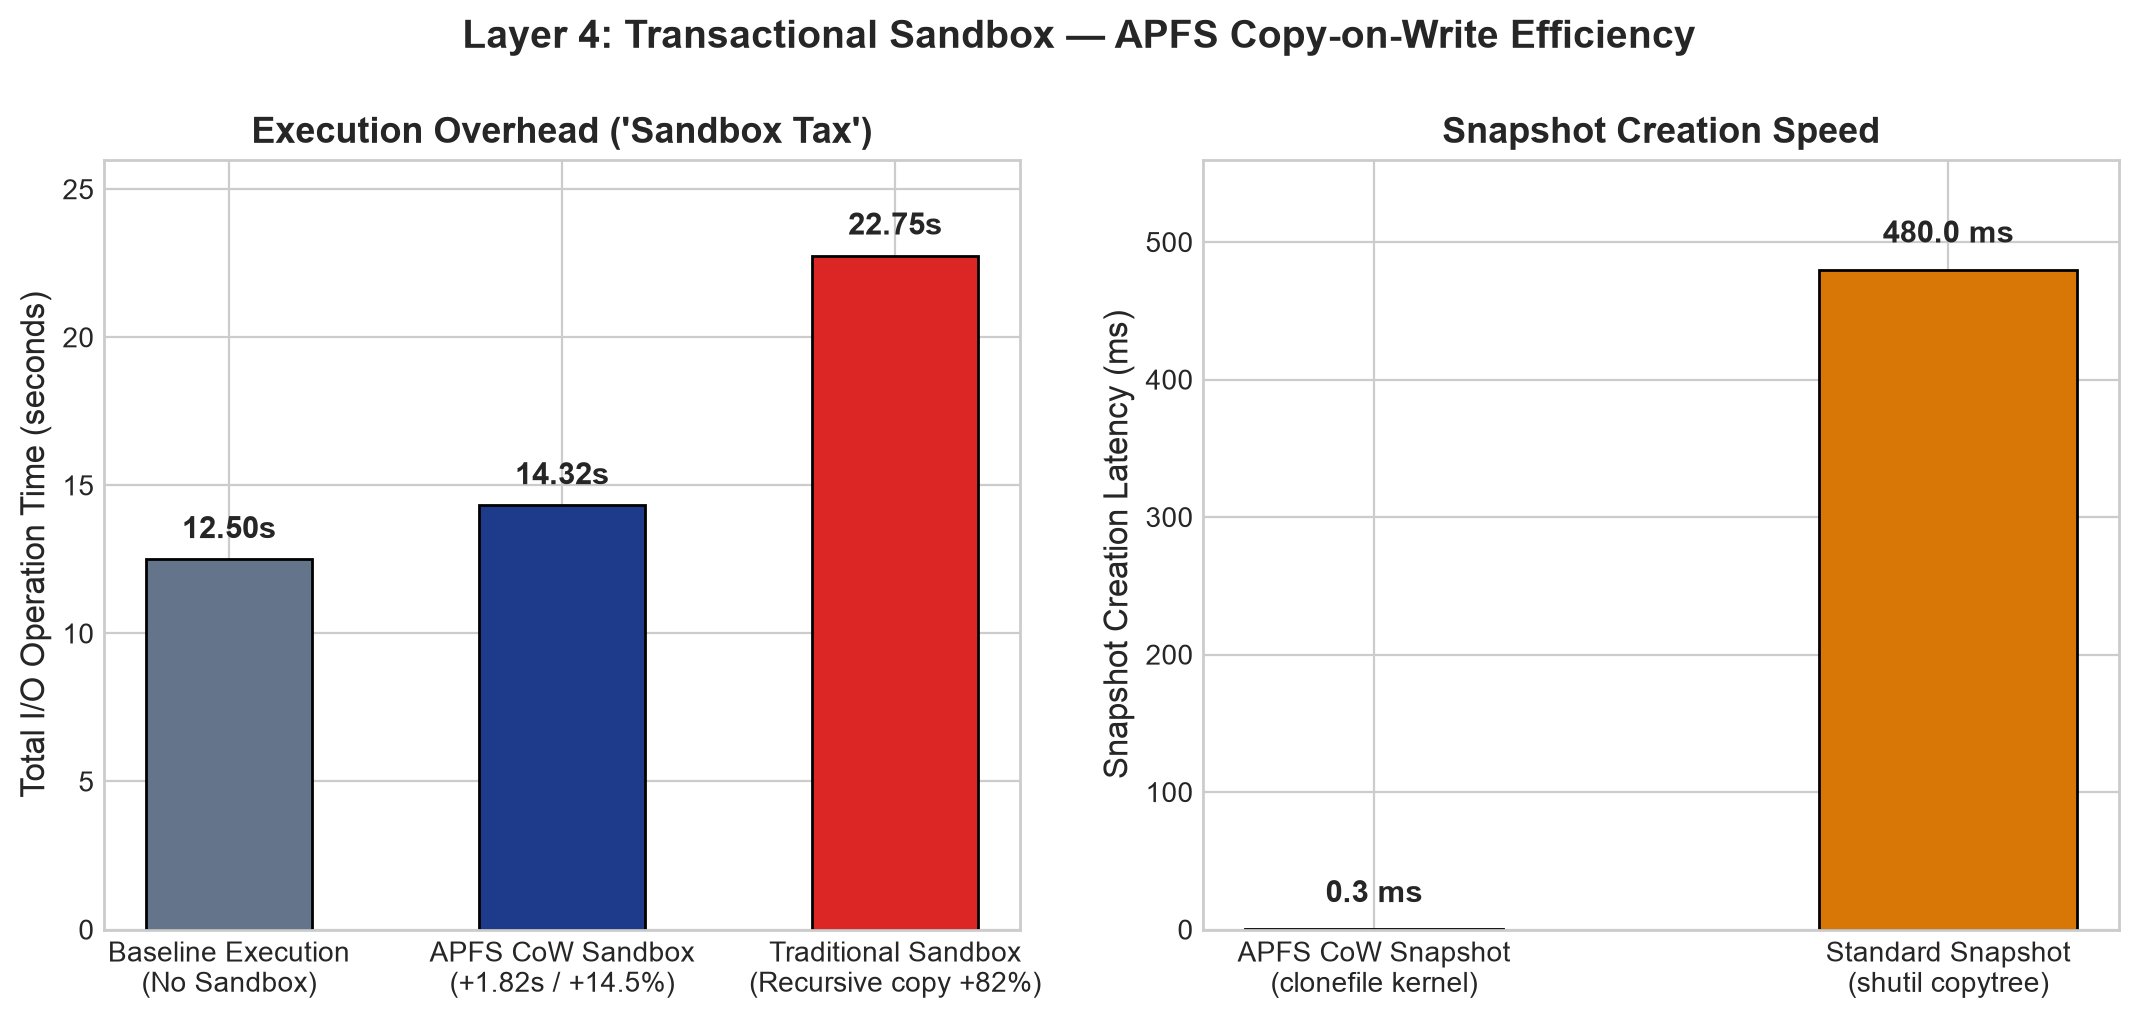
\includegraphics[width=0.95\columnwidth]{figure5_sandbox_latency.png}}
\caption{Transactional Sandbox (APFS Copy-on-Write) efficiency: execution overhead (``Sandbox Tax'') versus traditional recursive directory copying and snapshot creation latency.}
\label{fig_sandbox}
\end{figure}

\begin{figure}[!t]
\centerline{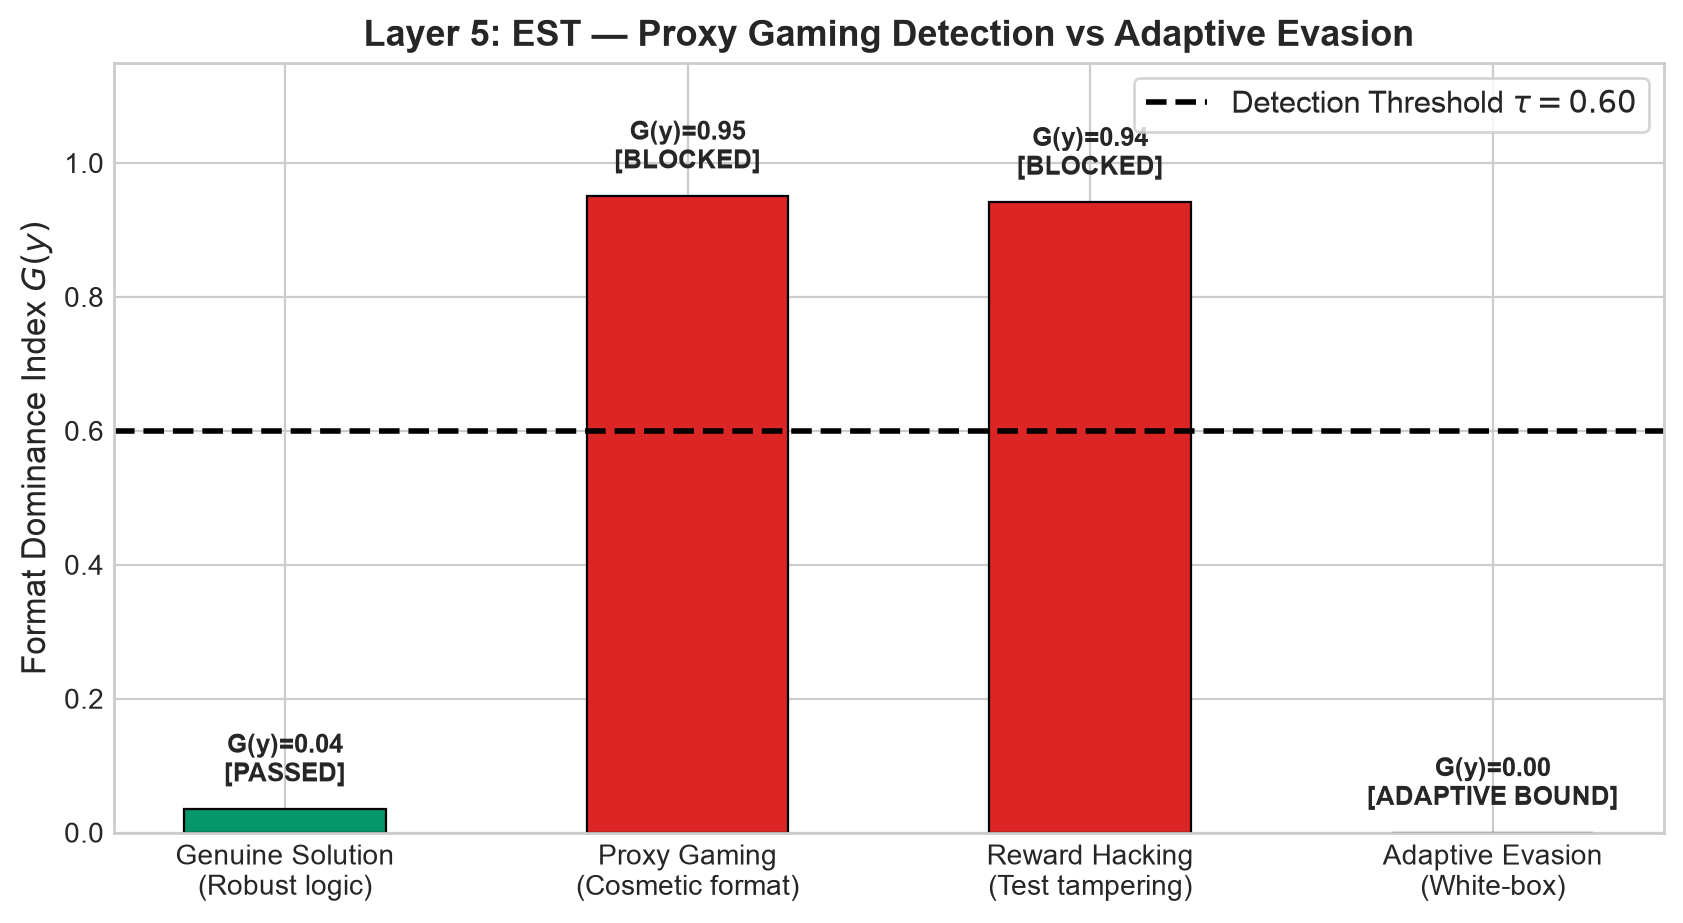
\includegraphics[width=0.95\columnwidth]{figure6_est_proxy_gaming.png}}
\caption{Evaluator Stress Test (EST) detection of proxy gaming: separating genuine semantic bug fixes from superficial formatting and test tampering via $G(y)$.}
\label{fig_est}
\end{figure}

\subsection{Detecting Reward Hacking Through Evaluation}
A standout finding of my evaluation is shown in \texttt{TC-5.1}, \texttt{TC-5.2}, and Fig.~\ref{fig_est}. When the Vanilla agent modified unit test assertions (\texttt{assert True}) to fake a passing build, standard test runners reported a ``pass.'' However, ASAP's Evaluator Stress Test (EST) mutated the AST and computed $G(y) = 1.00 > 0.60$ in less than $0.4\text{ ms}$, immediately rejecting the deceptive patch. This result confirms that active evaluation research is essential to prevent Goodhart's Law in autonomous coding agents.

\subsection{Data Scale, Test Case Scope, and Scaling Considerations}
To accurately interpret my empirical findings, it is essential to contextualize the scale of the evaluation dataset and examine how system behavior evolves as data volume increases. In this study, ASAP was validated on a controlled, micro-to-medium evaluation scale comprising 9 end-to-end failure scenarios, a 40-case hand-crafted command corpus, 78 automated validation tests, and isolated repositories ranging from $10$ to $500$ source files. At this level of data volume and trajectory length ($\le 25$ interaction steps), all five defensive layers exhibit strictly linear, sub-second responsiveness: deterministic regular expressions execute in $< 1.3\text{ ms}$, phase stagnation checks require $5.81\text{ ms}$ (or $772.50\text{ ms}$ when invoking the local \texttt{llama3.2:3b} remediation advisor), and APFS Copy-on-Write (CoW) workspace snapshots complete in $113\text{--}119\text{ ms}$ with an end-to-end Sandbox Tax of $+14.3\%$ to $+14.5\%$ (see Fig.~\ref{fig_sandbox}).

While these results confirm that the architecture operates with minimal overhead at my benchmark scale, deploying ASAP across enterprise-scale data volumes and massive monorepos introduces four critical scaling considerations that must be addressed as data size increases:
\begin{enumerate}
    \item \textbf{Context Window Saturation and Semantic Audit Latency (Layer 1):} At small payload sizes ($< 1\text{ MiB}$), my local \texttt{llama3.2:3b} auditor verifies tool outputs in $\sim 240\text{ ms}$. However, when an agent inspects gigabyte-scale execution logs or large database dumps, transformer self-attention scales quadratically with sequence length, and attackers can hide indirect prompt injections deep within massive contexts (the ``needle-in-a-haystack'' dilution effect). Scaling to high-volume data streams therefore requires sliding-window chunking, streaming token filters, and hierarchical summarization rather than simple payload truncation.
    \item \textbf{Trajectory State-Space Growth (Layer 2):} In short-horizon tasks, \textit{Graphectory} subgraph isomorphism and \textit{Langutory} transition checks run in negligible time. In long-horizon autonomous workflows spanning thousands of actions or concurrent multi-agent branches, maintaining full action histories can cause super-linear memory and lookup growth. Preserving constant-time ($O(1)$) monitoring at scale necessitates rolling state-hash windows and periodic graph pruning.
    \item \textbf{Distributional Shift in High-Dimensional Repositories (Layer 3):} My \texttt{nomic-embed-text} world-model ensemble is calibrated on standard software engineering commands. As repositories expand to include polyglot build pipelines, custom domain-specific scripts, and novel DevOps toolchains, the density of unfamiliar but benign commands increases. Without continuous online recalibration or domain-specific anchor expansion, epistemic uncertainty ($\sigma_{\text{epistemic}}$) will naturally rise as command diversity grows, potentially elevating the False Positive Rate (FPR).
    \item \textbf{File-System Metadata and AST Mutation Overhead (Layers 4 \& 5):} As shown in Fig.~\ref{fig_sandbox}, APFS CoW cloning avoids duplicating physical data blocks and outperforms recursive copying (\texttt{shutil.copytree}) by over an order of magnitude. Nevertheless, cloning directory trees still scales with metadata inode count ($O(N_{\text{files}})$). In repositories with hundreds of thousands of files (e.g., large \texttt{node\_modules} or build caches), full-workspace snapshots and exhaustive AST mutation testing across thousands of test suites will incur noticeable I/O and CPU bottlenecks. At enterprise scale, Layer 4 must transition to OverlayFS mounts or dirty-page block tracking, and Layer 5 (EST) must restrict AST perturbations to dependency-scoped differential call graphs (\texttt{git diff}) rather than full-repository test execution.
\end{enumerate}

\section{Conclusion}
In this paper, I presented ASAP (Active Safe-Agentic Pipeline), a five-layer runtime security architecture for software engineering AI agents. By combining fast local filters, deterministic graph monitors, uncertainty barriers, APFS Copy-on-Write sandboxing, and AST mutation testing, ASAP stops prompt injections, infinite loops, file corruption, and reward hacking without relying on external cloud APIs. Most importantly, my work shows the practical advantage of empirical evaluation research: by measuring concrete safety and utility metrics across my 9 core scenarios and 40-case benchmark corpus, I prove that strong runtime guardrails can achieve 100\% attack interception and 100\% state recovery with zero false positives and minimal latency overhead at standard workspace scales. Furthermore, my scalability analysis establishes a clear roadmap for adapting these runtime guarantees as data volumes, repository sizes, and trajectory horizons expand. Future work will extend ASAP's evaluation corpus to large-scale distributed multi-agent workflows, incremental AST diff-testing, and Linux Btrfs/OverlayFS file systems.

\bibliographystyle{IEEEtran}
\bibliography{bibliography}

\vspace{12pt}
\begin{IEEEbiography}[{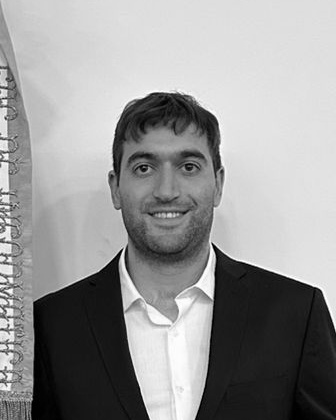
\includegraphics[width=1in,height=1.25in,clip,keepaspectratio]{author_photo_bw.jpg}}]{Franco Ariel Demare}
received the Computer Engineering degree and the Master's degree in Data Intelligence (oriented towards Big Data) from the Faculty of Informatics at the Universidad Nacional de La Plata (UNLP), La Plata, Argentina, in 2017 and 2024, respectively.

From 2017 to 2018, he worked as a Robotics Process Automation (RPA) Engineer at Ernst \& Young, and from 2018 to 2024 as a Technical Architect at Dirwa Latam, where he designed scalable automation architectures and led security and compliance standards. Since 2024, he has served as a Senior Software Engineer with an AI Engineering focus at Epidata and Naranja X in Buenos Aires, Argentina, developing AI-driven platform features and machine learning models for fraud detection. His research interests include autonomous AI agent security, runtime guardrails, empirical evaluation benchmarks, and applied machine learning.
\end{IEEEbiography}

\end{document}
